\documentclass[compress]{beamer}
\usepackage{irbookslide}
\usepackage{irilmenau2}
\usepackage{tikz}
\usepackage{url}
\usepackage{ifxetex}
%\RequireXeTeX
\usepackage{fontspec} % zahteva paket euenc
\usepackage{xunicode}
\usepackage{xltxtra}
\usepackage{polyglossia}
\usepackage{minted}
\usepackage[noend]{algorithmic}
\renewcommand{\algorithmicrequire}{\textbf{Input:}}
\renewcommand{\algorithmicensure}{\textbf{Output:}}
\renewcommand{\algorithmiccomment}[1]{\hfill \{\myred{#1}\}}
\usepackage{xcolor,colortbl}
\usepackage{textcomp}
\usepackage{unicode-math}
%\usepackage{hyphenat}
%\setdefaultlanguage[script=Latin]{serbian}

\title{Obrada teksta}
\author{\textcopyright \ \ Goodrich, Tamassia, Goldwasser}
\institute{Katedra za informatiku, Fakultet tehničkih nauka, Univerzitet u
Novom Sadu}
\date{2014.}
\subject{Predavanja sa ASP}

\begin{document}

\frame{\titlepage}

\section[Stringovi]{Stringovi}

\begin{frame}[fragile]
  \frametitle{String}
  \begin{itemize}
    \item \myred{string} je niz karaktera
    \item primeri stringova:
    \begin{itemize}
      \item Python program
      \item HTML dokument
      \item DNK sekvenca
      \item digitalna slika
    \end{itemize}
    \item \myred{alfabet} $\Sigma$ je skup mogućih karaktera za familiju stringova
    \item primeri alfabeta:
    \begin{itemize}
      \item ASCII
      \item Unicode
      \item \{0, 1\}
      \item \{A, C, G, T\}
    \end{itemize}
  \end{itemize}
\end{frame}

\begin{frame}[fragile]
  \frametitle{String}
  \begin{itemize}
    \item neka je $P$ string dužine $m$
    \begin{itemize}
      \item \myred{podstring} $P[i..j]$ od $P$ je podsekvenca od $P$ koja sadrži
      karaktere sa rangom između $i$ i $j$
      \item \myred{prefiks} od $P$ je podstring tipa $P[0..i]$
      \item \myred{sufiks} od $P$ je podstring tipa $P[i..m-1]$
    \end{itemize}
    \item za date stringove $T$ (tekst) i $P$ (šablon, \textit{pattern})
    \textit{pattern matching} problem je pronalaženje podstringa
    od $T$ koji je jednak $P$
    \item primene:
    \begin{itemize}
      \item editori teksta
      \item mašine za pretragu (\textit{search engines})
      \item bioinformatika
    \end{itemize}
  \end{itemize}
\end{frame}

\section[GS]{Gruba sila}

\begin{frame}[fragile]
  \frametitle{Nalaženje podstringa grubom silom}
  \begin{itemize}
    \item nalaženje \myred{grubom silom} (\textit{brute force}) poredi šablon
    $P$ sa tekstom $T$ za svaki mogući položaj $P$ u odnosu na $T$ sve dok se
    \begin{itemize}
      \item ne pronađe poklapanje
      \item ne testiraju sve pozicije
    \end{itemize}
    \item gruba sila radi u $O(nm)$ vremenu
    \item primer najgoreg slučaja:
    \begin{itemize}
      \item $T = aaa \ldots ah$
      \item $P = aaah$
      \item može da se pojavi u slikama i DNK sekvencama
      \item retko u tekstovima
    \end{itemize}
  \end{itemize}
\end{frame}

\begin{frame}[fragile,shrink]
  \frametitle{Nalaženje podstringa grubom silom}
  \myred{BruteForceMatch}($T, P$)
  \begin{algorithmic}
    \REQUIRE tekst $T$ dužine $n$ i šablon $P$ dužine $m$
    \ENSURE indeks početka podstringa u $T$ jednakog $P$ ili -1 ako nije pronađen
    \FOR{$i \leftarrow 0$ \TO $n-m$}
      \STATE $j \leftarrow 0$  \COMMENT{testiramo položaj i}
      \WHILE{$j<m \land T[i+j]=P[j]$}
        \STATE $j \leftarrow j+1$
        \IF{$j=m$}
          \RETURN $i$ \COMMENT{poklapanje na $i$}
        \ELSE
          \STATE break
        \ENDIF
      \ENDWHILE
    \ENDFOR
    \RETURN -1 \COMMENT{nije pronađen}
  \end{algorithmic}    
\end{frame}

\begin{frame}[fragile,shrink=18]
  \frametitle{Gruba sila u Pythonu}
\begin{minted}[linenos=false]{python}
def find_brute_force(T, P):
  """Return the lowest index of T at which
     substring P begins (or else -1)."""
  n, m = len(T), len(P)  # introduce convenient notations
  for i in range(n-m+1): # try every potential starting index within T
    k = 0                # an index into pattern P
    while k < m and T[i + k] == P[k]: # kth character of P matches
      k += 1
    if k == m:           # if we reached the end of pattern,
      return i           # substring T[i:i+m] matches P
  return -1              # failed to find a match starting with any i
\end{minted}
\end{frame}

\section[BM]{Boyer-Moore}

\begin{frame}[fragile]
  \frametitle{Boyer-Moore}
  \begin{itemize}
    \item \myred{Boyer-Moore} algoritam se zasniva na dve heuristike
    \begin{itemize}
      \item \myred{ogledalo}: poredi $P$ sa podsekvencom u $T$ idući unazad
      \item \myred{skok}: ako se razlika otkrije u $T[i]=c$
      \begin{itemize}
        \item ako $P$ sadrži $c$, pomeri $P$ tako da se $T[i]$ poklopi sa
        poslednjom pojavom $c$ u $P$
        \item inače pomeri $P$ tako da se poklope $P[0]$ i $T[i+1]$
      \end{itemize}
    \end{itemize}
  \end{itemize}
  \begin{center}
    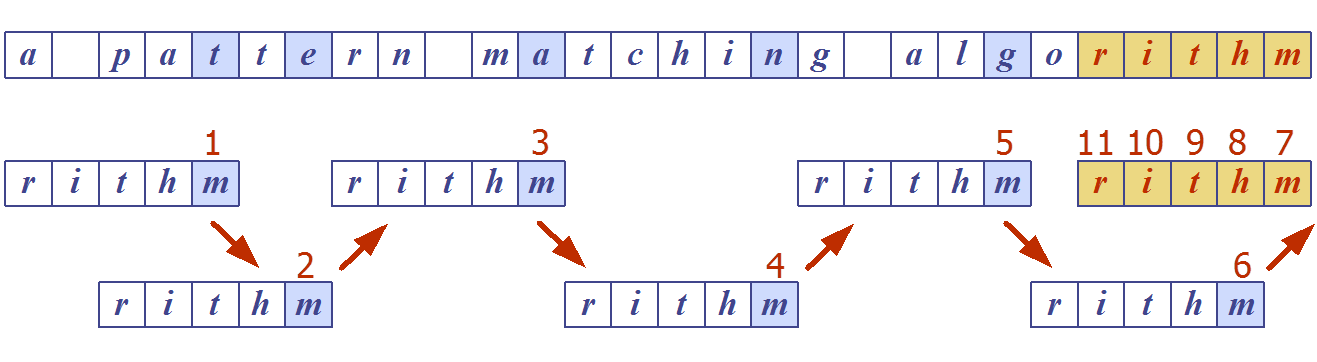
\includegraphics[width=11cm]{asp-13-pic01.png}
  \end{center}
\end{frame}

\begin{frame}[fragile]
  \frametitle{Boyer-Moore: funkcija poslednjeg pojavljivanja}
  \begin{itemize}
    \item \myred{Boyer-Moore} algoritam formira \myred{last occurence} funkciju $L$ koja
    mapira alfabet $\Sigma$ na cele brojeve gde je $L(c)$ definisano kao
    \begin{itemize}
      \item najveći indeks $i$ takav da $P[i]=c$
      \item $-1$ ako takvog indeksa nema
    \end{itemize}
    \item primer: $\Sigma = \{a,b,c,d\} \quad P = abacab$
  \end{itemize}
  \begin{center}
    \begin{tabular}{c||c|c|c|c}
    $c$ & $a$ & $b$ & $c$ & $d$ \\ \hline
    $L(c)$ & $4$ & $5$ & $3$ & $-1$ \\
    \end{tabular}
  \end{center}
  \begin{itemize}
    \item može se predstaviti kao niz indeksiran numeričkim kodovima karaktera
    \item može se izračunati za $O(m+s)$ vreme gde je $m$ dužina $P$ a $s$ je veličina $\Sigma$
  \end{itemize}
\end{frame}

\begin{frame}[fragile,shrink]
  \frametitle{Boyer-Moore algoritam}
  \myred{BoyerMooreMatch}($T, P, \Sigma$)
  \begin{algorithmic}
    \STATE $L \leftarrow$ lastOccurence($P,\Sigma$)
    \STATE $i \leftarrow m-1$ \COMMENT{indeks u $T$}
    \STATE $j \leftarrow m-1$ \COMMENT{indeks u $P$}
    \REPEAT
      \IF{$T[i]=P[j]$}
        \IF{$j=0$}
          \RETURN $i$ \COMMENT{poklapanje na i}
        \ELSE
          \STATE $i \leftarrow i-1$
          \STATE $j \leftarrow j-1$
        \ENDIF
      \ELSE
        \STATE $l \leftarrow L[T[i]]$ \COMMENT{indeks poslednjeg pojavljivanja}
        \STATE $i \leftarrow i + m - \min(j, 1+l)$ \COMMENT{dva slučaja za skok}
        \STATE $j \leftarrow m-1$
      \ENDIF
    \UNTIL{$i>n-1$}
    \RETURN $-1$ \COMMENT{nije pronađen}
  \end{algorithmic}    
\end{frame}

\begin{frame}[fragile]
  \frametitle{Boyer-Moore}
  \begin{center}
    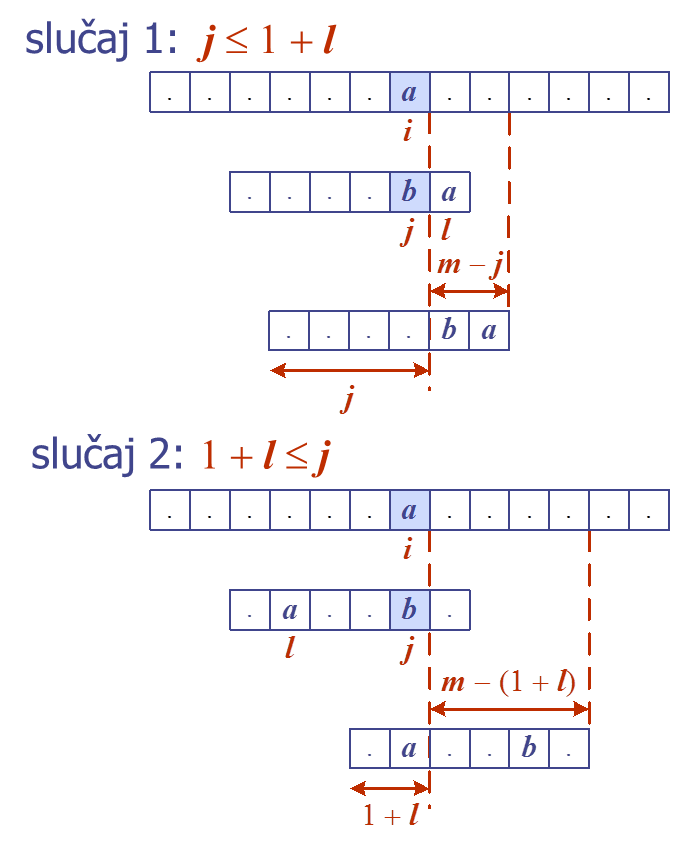
\includegraphics[width=6cm]{asp-13-pic02.png}
  \end{center}
\end{frame}

\begin{frame}[fragile]
  \frametitle{Boyer-Moore: primer}
  \begin{center}
    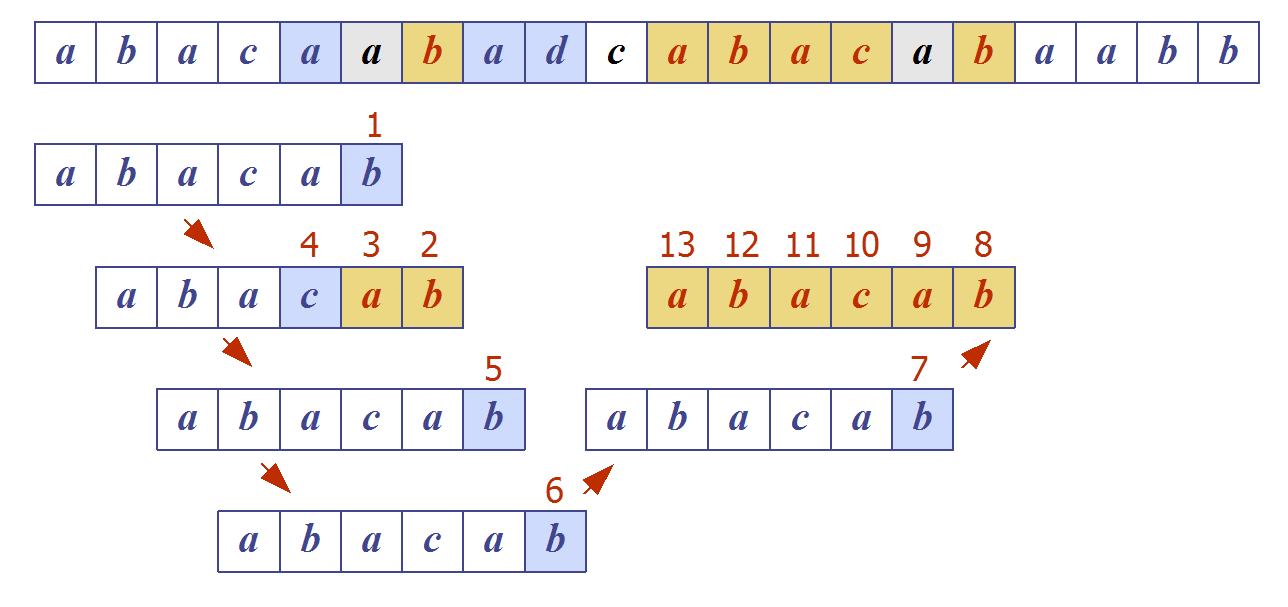
\includegraphics[width=11cm]{asp-13-pic03.png}
  \end{center}
\end{frame}

\begin{frame}[fragile]
  \frametitle{Boyer-Moore: analiza}
  \begin{columns}
    \begin{column}[t]{6cm}
      \begin{itemize}
        \item Boyer-Moore je $O(nm+s)$
        \item primer najgoreg slučaja:
        \begin{itemize}
          \item $T = aaa \ldots a$
          \item $P = baaa$
        \end{itemize}
        \item najgori slučaj nije verovatan u tekstovima
        \item znatno brži od grube sile za tekstove na prirodnom jeziku
      \end{itemize}
    \end{column}
    \begin{column}[t]{6cm}
      \begin{center}
        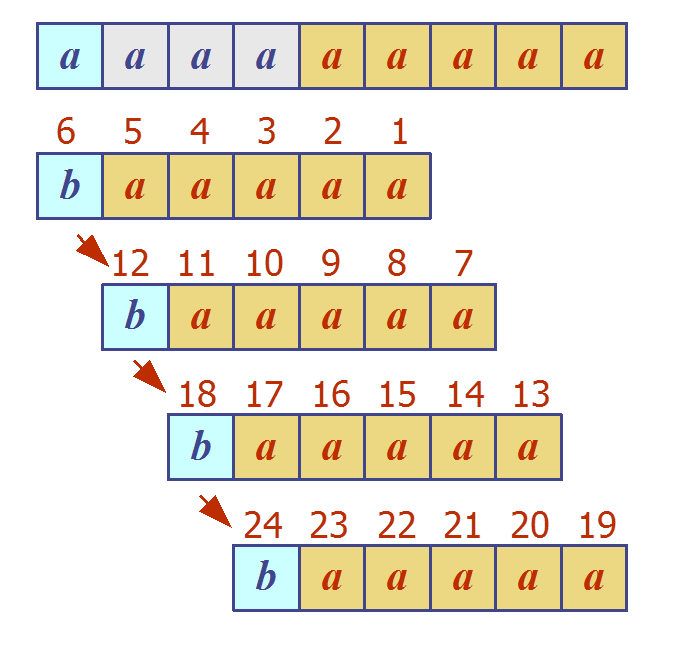
\includegraphics[width=6cm]{asp-13-pic04.png}
      \end{center}
    \end{column}
  \end{columns}
\end{frame}

\begin{frame}[fragile,shrink]
  \frametitle{Boyer-Moore u Pythonu}
\begin{minted}[linenos=false]{python}
def find_boyer_moore(T, P):
  """Return the lowest index of T at which substring P begins (or else -1)."""
  n, m = len(T), len(P)                   # introduce convenient notations
  if m == 0: return 0                     # trivial search for empty string
  last = {}                               # build 'last' dictionary
  for k in range(m):
    last[ P[k] ] = k                      # later occurrence overwrites
  # align end of pattern at index m-1 of text
  i = m-1                                 # an index into T
  k = m-1                                 # an index into P
  while i < n:
    if T[i] == P[k]:                      # a matching character
      if k == 0:
        return i                          # pattern begins at index i of text
      else:
        i -= 1                            # examine previous character
        k -= 1                            # of both T and P
    else:
      j = last.get(T[i], -1)              # last(T[i]) is -1 if not found
      i += m - min(k, j + 1)              # case analysis for jump step
      k = m - 1                           # restart at end of pattern
  return -1
\end{minted}
\end{frame}

\section[KMP]{Knuth-Morris-Pratt}

\begin{frame}[fragile]
  \frametitle{Knuth-Morris-Pratt}
  \begin{columns}
    \begin{column}[t]{6cm}
      \begin{itemize}
        \item \myred{Knuth-Morris-Pratt} poredi tekst sa šablonom \textbf{sleva
        u desno} ali pomera šablon pametnije od grube sile
        \item kada se nađe razlika, koliko \textbf{najviše} možemo pomeriti
        šablon da izbegnemo suvišna poređenja?
        \item odgovor: najveći prefiks $P[0..j]$ koji je sufiks $P[1..j]$
      \end{itemize}
    \end{column}
    \begin{column}[t]{6cm}
      \begin{center}
        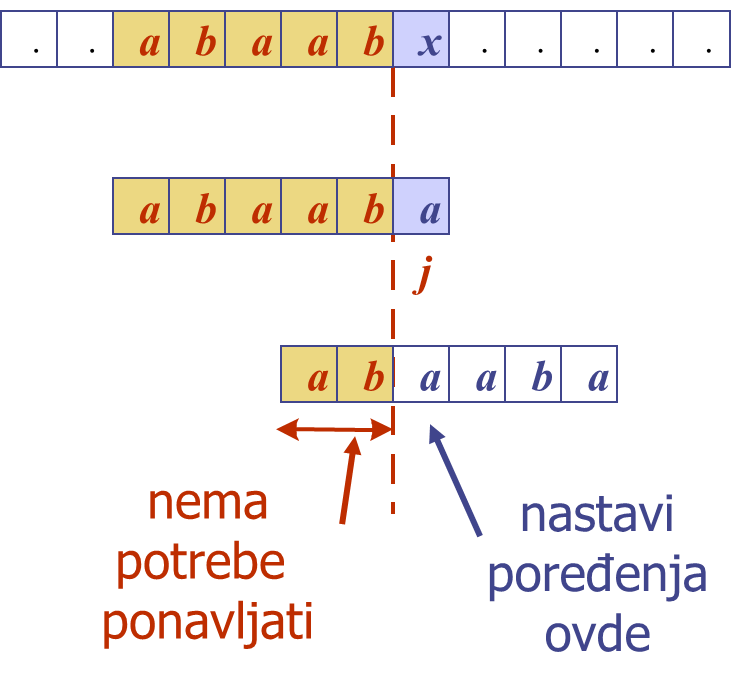
\includegraphics[width=6cm]{asp-13-pic05.png}
      \end{center}
    \end{column}
  \end{columns}
\end{frame}

\begin{frame}[fragile]
  \frametitle{KMP: funkcija neuspeha}
  \begin{columns}
    \begin{column}[t]{6cm}
      \begin{itemize}
        \item KMP analizira šablon da pronađe njegove prefikse unutar samog
        šablona
        \item \myred{funkcija neuspeha} $F(j)$ je veličina najvećeg prefiksa
        $P[0..j]$ takvog da je ujedno i sufiks $P[1..j]$
        \item razlika KMP i GS: ako nema poklapanja za $P[j] \neq T[i]$ pomeramo
        $j \leftarrow F(j-1)$
      \end{itemize}
    \end{column}
    \begin{column}[t]{6cm}
      \begin{center}
        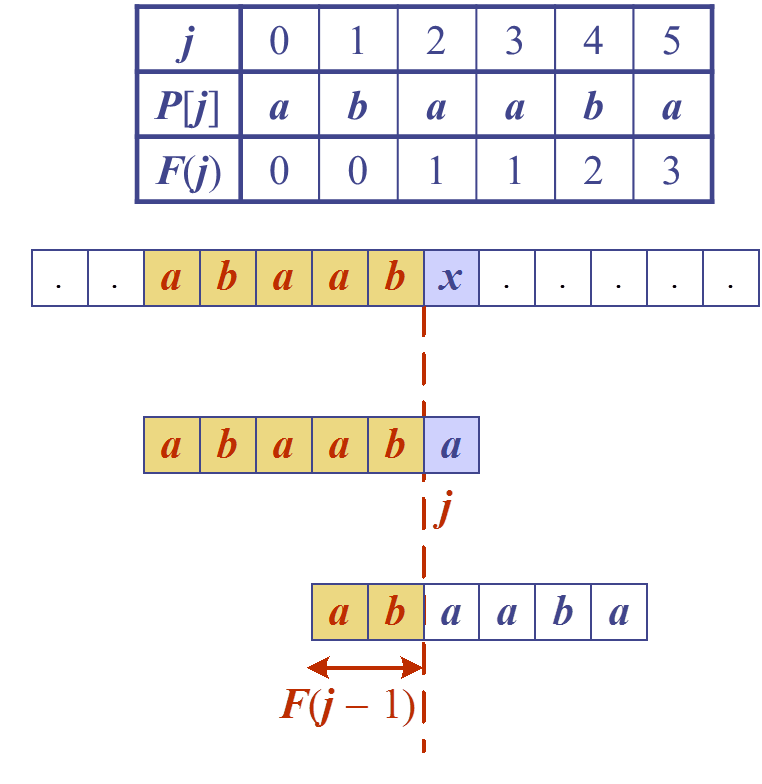
\includegraphics[width=6cm]{asp-13-pic06.png}
      \end{center}
    \end{column}
  \end{columns}
\end{frame}

\begin{frame}[fragile,shrink=12]
  \frametitle{Knuth-Morris-Pratt algoritam}
  \begin{columns}
    \begin{column}[t]{6cm}
      \begin{itemize}
        \item funkcija neuspeha se može prikazati nizom koji se izračuna za $O(m)$
        \item u svakoj iteraciji petlje, ili
        \begin{itemize}
          \item $i$ se poveća za $1$, ili
          \item pomeraj $i-j$ se poveća za najmanje $1$ (primeti da $F(j-1)<j$)
        \end{itemize}
        \item $\Rightarrow$ nema više od $2n$ iteracija u petlji
        \item $\Rightarrow$ KMP je $O(m+n)$
      \end{itemize}
    \end{column}
    \begin{column}[t]{6cm}
      \myred{KMPMatch}($T, P$)
      \begin{algorithmic}
        \STATE $F \leftarrow$ failureFunction($P$)
        \STATE $i \leftarrow 0$
        \STATE $j \leftarrow 0$
        \WHILE{$i<n$}
          \IF{$T[i]=P[j]$}
            \IF{$j=m-1$}
              \RETURN $i-j$ \COMMENT{poklapanje}
            \ELSE
              \STATE $i \leftarrow i+1$
              \STATE $j \leftarrow j+1$
            \ENDIF
          \ELSE
            \IF{$j>0$}
              \STATE $j \leftarrow F[j-1]$
            \ELSE
              \STATE $i \leftarrow i + 1$
            \ENDIF
          \ENDIF
        \ENDWHILE
        \RETURN $-1$ \COMMENT{nije pronađen}
      \end{algorithmic}    
    \end{column}
  \end{columns}
\end{frame}

\begin{frame}[fragile,shrink=12]
  \frametitle{KMP: izračunavanje funkcije neuspeha}
  \begin{columns}
    \begin{column}[t]{6cm}
      \begin{itemize}
        \item funkcija neuspeha se može prikazati nizom koji se izračuna za $O(m)$
        \item slično kao i sam KMP algoritam
        \item u svakoj iteraciji petlje, ili
        \begin{itemize}
          \item $i$ se poveća za $1$, ili
          \item pomeraj $i-j$ se poveća za najmanje $1$ (primeti da $F(j-1)<j$)
        \end{itemize}
        \item $\Rightarrow$ nema više od $2n$ iteracija u petlji
      \end{itemize}
    \end{column}
    \begin{column}[t]{6cm}
      \myred{failureFunction}($P$)
      \begin{algorithmic}
        \STATE $F[0] \leftarrow 0$
        \STATE $i \leftarrow 1$
        \STATE $j \leftarrow 0$
        \WHILE{$i<m$}
          \IF{$P[i]=P[j]$}
            \STATE \COMMENT{poklapa se $j+1$ znakova}
            \STATE $F[i] \leftarrow j+1$
            \STATE $i \leftarrow i+1$
            \STATE $j \leftarrow j+1$
          \ELSIF{$j>0$}
            \STATE \COMMENT{koristi $F$ da pomeriš $P$}
            \STATE $j \leftarrow F[j-1]$
          \ELSE
            \STATE $F[0] \leftarrow 0$ \COMMENT{nema poklapanja}
            \STATE $i \leftarrow i + 1$
          \ENDIF
        \ENDWHILE
      \end{algorithmic}    
    \end{column}
  \end{columns}
\end{frame}

\begin{frame}[fragile]
  \frametitle{Knuth-Morris-Pratt: primer}
  \begin{center}
    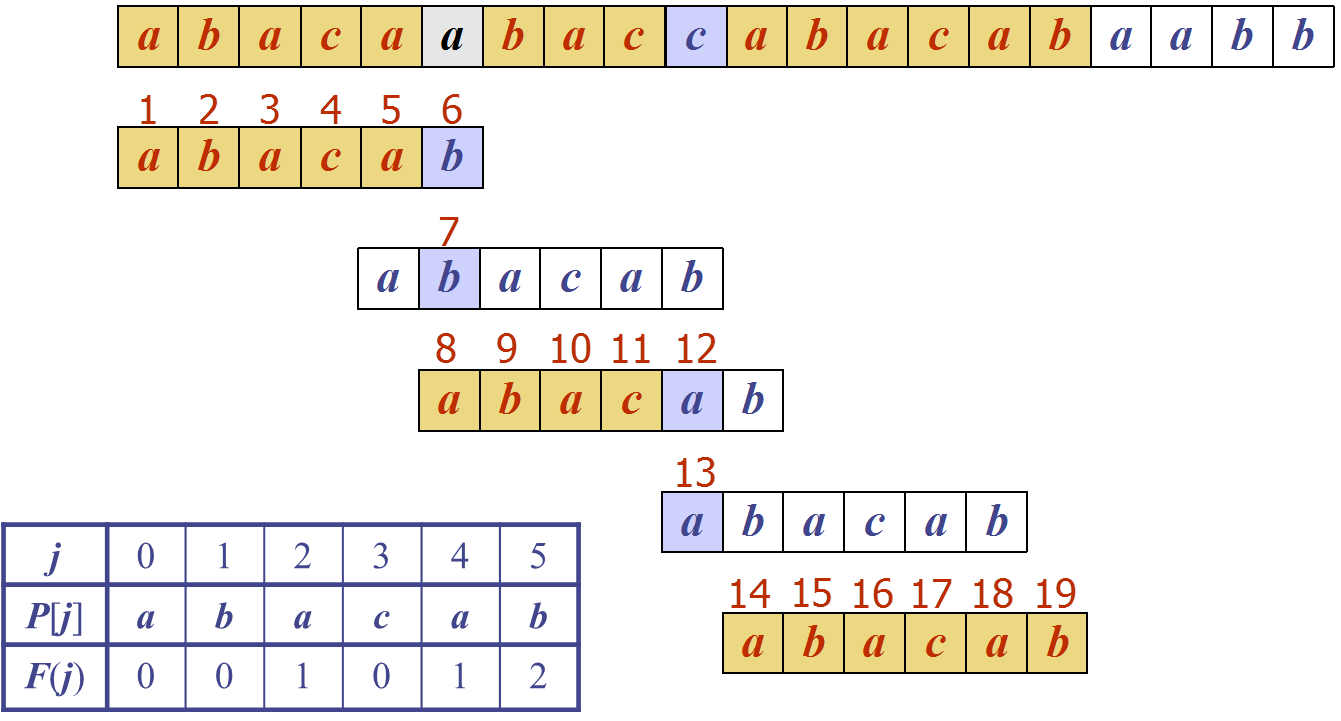
\includegraphics[width=11cm]{asp-13-pic07.png}
  \end{center}
\end{frame}

\begin{frame}[fragile,shrink]
  \frametitle{Knuth-Morris-Pratt u Pythonu $_1$}
\begin{minted}[linenos=false]{python}
def find_kmp(T, P):
  """Return the lowest index of T
     at which substring P begins (or else -1)."""
  n, m = len(T), len(P)       # introduce convenient notations
  if m == 0: return 0         # trivial search for empty string
  fail = compute_kmp_fail(P)  # rely on utility to precompute
  j = 0                       # index into text
  k = 0                       # index into pattern
  while j < n:
    if T[j] == P[k]:          # P[0:1+k] matched thus far
      if k == m - 1:          # match is complete
        return j - m + 1           
      j += 1                  # try to extend match
      k += 1
    elif k > 0:                    
      k = fail[k-1]           # reuse suffix of P[0:k]
    else:
      j += 1
  return -1                   # reached end without match
\end{minted}
\end{frame}

\begin{frame}[fragile,shrink=12]
  \frametitle{Knuth-Morris-Pratt u Pythonu $_2$}
\begin{minted}[linenos=false]{python}
def compute_kmp_fail(P):
  """Utility that computes and returns KMP 'fail' list."""
  m = len(P)
  fail = [0] * m    # by default, presume overlap of 0 everywhere
  j = 1
  k = 0
  while j < m:        # compute f(j) during this pass, if nonzero
    if P[j] == P[k]:  # k + 1 characters match thus far
      fail[j] = k + 1
      j += 1
      k += 1
    elif k > 0:       # k follows a matching prefix
      k = fail[k-1]
    else:             # no match found starting at j
      j += 1
  return fail
\end{minted}
\end{frame}

\section[Din prog]{Dinamičko programiranje}

\begin{frame}[fragile]
  \frametitle{Dinamičko programiranje}
  \begin{columns}
    \begin{column}[t]{6cm}
      \begin{itemize}
        \item \myred{dinamičko programiranje} je pristup dizajnu algoritama
        \item prvo primer: množenje matrica
        $$ C[i,j] = \sum_{k=0}^{e-1} A[i,k]\cdot B[k,j]$$
        \item vreme je $O(d\cdot e\cdot f)$
      \end{itemize}
    \end{column}
    \begin{column}[t]{6cm}
      \begin{center}
        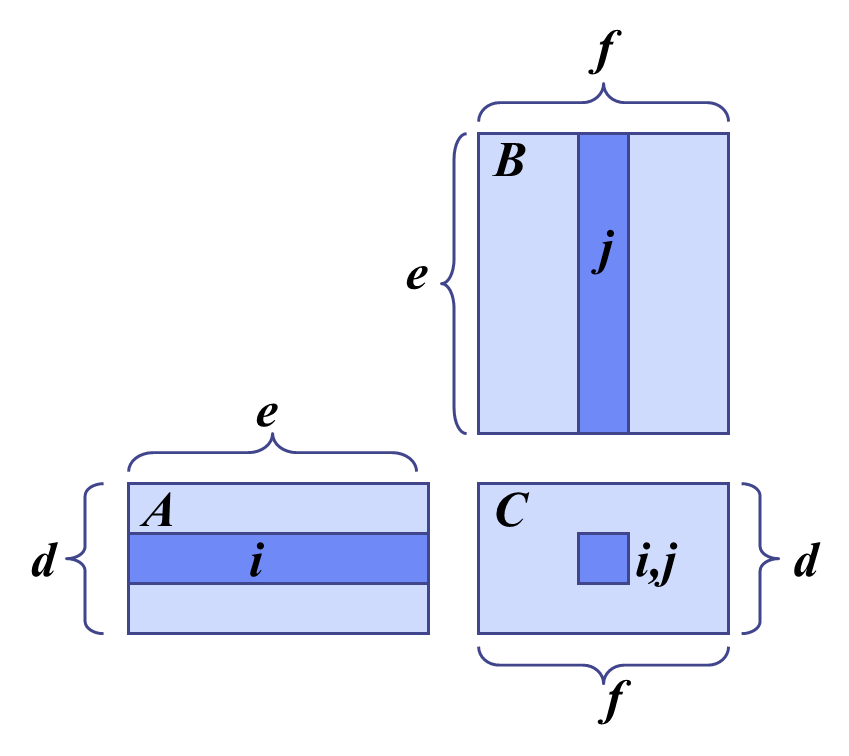
\includegraphics[width=6cm]{asp-13-pic08.png}
      \end{center}
    \end{column}
  \end{columns}
\end{frame}

\begin{frame}[fragile]
  \frametitle{Množenje matrica}
  \begin{itemize}
    \item računamo $A=A_0 \cdot A_{1}\cdot \ldots\cdot A_{n-1}$
    \item $A_{i}$ ima dimenzije $d_{i}\times d_{i+1}$
    \item koji redosled množenja izabrati?
    \item primer:
    \begin{itemize}
      \item $B$ je $3\times 100$
      \item $C$ je $100\times 5$
      \item $D$ je $5\times 5$
      \item $(B\cdot C)\cdot D$ traži 1500+75 = 1575 operacija
      \item $B\cdot (C\cdot D)$ traži 1500+2500 = 4000 operacija
    \end{itemize}
  \end{itemize}
\end{frame}

\begin{frame}[fragile]
  \frametitle{Raspoređivanje zagrada / gruba sila}
  \begin{itemize}
    \item traženje rešenja grubom silom: isprobati sve moguće 
    kombinacije zagrada za $A=A_0 \cdot A_{1}\cdot \ldots\cdot A_{n-1}$ 
    \item izračunati broj operacija za svaku
    \item i izabrati najbolju
    \item vreme izvršavanja:
    \begin{itemize}
      \item broj mogućih rasporeda zagrada je jednak broju različitih 
      binarnih stabala sa $n$ čvorova
      \item \textbf{eksponencijalna} zavisnost!
      \item tzv. Katalanov broj, iznosi skoro $4^n$
    \end{itemize}
  \end{itemize}
\end{frame}

\begin{frame}[fragile]
  \frametitle{Pohlepni pristup}
  \begin{itemize}
    \item ideja \#1: ponavljaj izbor onog proizvoda koji će imati \textbf{najviše} operacija
    \item protiv-primer:
    \begin{itemize}
      \item $A$ je $10\times 5$
      \item $B$ je $5\times 10$
      \item $C$ je $10\times 5$
      \item $D$ je $5\times 10$
      \item ideja \#1 daje $(A\cdot B)\cdot (C\cdot D)$, \\ tj. 500+1000+500 = 2000 operacija
      \item $A\cdot ((B\cdot C)\cdot D)$ je 500+250+250 = 1000 operacija
    \end{itemize}
  \end{itemize}
\end{frame}

\begin{frame}[fragile]
  \frametitle{Pohlepni pristup}
  \begin{itemize}
    \item ideja \#2: ponavljaj izbor onog proizvoda koji će imati \textbf{najmanje} operacija
    \item protiv-primer:
    \begin{itemize}
      \item $A$ je $101\times 11$
      \item $B$ je $11\times 9$
      \item $A$ je $9\times 100$
      \item $B$ je $100\times 99$
      \item ideja \#2 daje $A\cdot ((B\cdot C)\cdot D)$, \\ tj. 109989+9900+108900 = 228789 operacija
      \item $(A\cdot B)\cdot (C\cdot D)$ je 9999+89991+89100 = 189090 operacija
    \end{itemize}
    \item pohlepni pristup ne donosi optimalan izbor
  \end{itemize}
\end{frame}

\begin{frame}[fragile]
  \frametitle{,,Rekurzivni`` pristup}
  \begin{itemize}
    \item definišemo \myred{potprobleme}
    \begin{itemize}
      \item nađi najbolji raspored zagrada za $A_{i}\cdot A_{i+1}\cdot \ldots A_{j}$
      \item neka je $N_{i,j}$ broj operacija za ovaj potproblem
      \item optimalno rešenje za ceo problem je $N_{0,n-1}$
    \end{itemize}
    \item \myred{optimalnost potproblema}: optimalno rešenje se može 
    dobiti pomoću optimalnih potproblema
    \begin{itemize}
      \item mora postojati poslednje množenje (koren stabla izraza) za 
      optimalno rešenje
      \item neka je to na $i$-tom indeksu: $(A_{0}\cdot \ldots \cdot A_{i})\cdot (A_{i+1}\cdot \ldots \cdot A_{n-1})$
      \item optimalno rešenje za ceo problem $N_{0,n-1}$ je suma dva optimalna potproblema plus poslednje množenje
      \item ako bi optimalno rešenje imalo bolje potprobleme, ne bi bilo optimalno
    \end{itemize}
  \end{itemize}
\end{frame}

\begin{frame}[fragile]
  \frametitle{Karakteristična jednačina}
  \begin{itemize}
    \item globalni optimum se definiše pomoću optimalnih potproblema u 
    zavisnosti od indeksa poslednjeg množenja
    \item razmotrimo sve moguće vrednosti tog indeksa
    \begin{itemize}
      \item $A_{i}$ je dimenzije $d_{i}\times d_{i+1}$
      \item karakteristična jednačina za $N_{i,j}$ je:
      $$ N_{i,j} = \min_{i\leq k<j}\{ N_{i,k} + N_{k+1,j} + d_{i} d_{k+1} d_{j+1}\}$$
    \end{itemize}
    \item potproblemi nisu nezavisni, nego se \myred{preklapaju}
  \end{itemize}
\end{frame}

\begin{frame}[fragile]
  \frametitle{Algoritam dinamičkog programiranja}
  \begin{itemize}
    \item pošto se problemi preklapaju, nećemo koristiti rekurziju
    \item konstruisaćemo optimalne potprobleme od dole na gore (\textit{bottom-up})
    \item $N_{i,i}$ je lako, počnemo od njih
    \item onda pređemo na potprobleme dužine 2, 3, \ldots{}
    \item vreme izvršavanja je $O(n^3)$
  \end{itemize}
\end{frame}

\begin{frame}[fragile,shrink]
  \frametitle{Algoritam dinamičkog programiranja}
  \myred{matrixChain}($S$)
  \begin{algorithmic}
    \REQUIRE sekvenca $S$ matrica koje treba pomnožiti
    \ENSURE broj operacija u optimalnom rasporedu zagrada
    \FOR{$i \leftarrow 0$ \TO $n-1$}
      \STATE $N_{i,i} \leftarrow 0$
    \ENDFOR
    \FOR{$b \leftarrow 1$ \TO $n-1$}
      \FOR{$i \leftarrow 0$ \TO $n-b-1$}
        \STATE $j \leftarrow i+b$
        \STATE $N_{i,j} \leftarrow +\infty$
        \FOR{$k \leftarrow i$ \TO $j-1$}
          \STATE $N_{i,j} \leftarrow \min_{k} \{ N_{i,k} + N_{k+1,j} + d_{i} d_{k+1} d_{j+1}\}$
        \ENDFOR
      \ENDFOR
    \ENDFOR
  \end{algorithmic}    
\end{frame}

\begin{frame}[fragile,shrink=15]
  \frametitle{Python implementacija}
\begin{minted}[linenos=false]{python}
def matrix_chain(d):
  """Return solution to the matrix chain problem.

  d is a list of n+1 numbers describing the dimensions of a chain of
  n matrices such that kth matrix has dimensions d[k]-by-d[k+1].
 
  Return an n-by-n table such that N[i][j] represents the minimum 
  number of multiplications needed to compute the product of Ai 
  through Aj inclusive.
  """
  n = len(d) - 1                  # number of matrices
  N = [[0] * n for i in range(n)] # initialize n-by-n result to zero
  for b in range(1, n):           # number of products in subchain
    for i in range(n-b):          # start of subchain
      j = i + b                   # end of subchain
      N[i][j] = min(N[i][k] + N[k+1][j] + d[i]*d[k+1]*d[j+1] \
        for k in range(i,j))
  return N
\end{minted}
\end{frame}

\begin{frame}[fragile,shrink]
  \frametitle{Vizuelizacija algoritma}
  \begin{columns}
    \begin{column}[t]{6cm}
      \begin{itemize}
        \item bottom-up prvo popuni dijagonalu
        \item $N_{i,j}$ se dobija na osnovu vrednosti iz $i$-tog reda i 
        $j$-te kolone
        \item popunjavanje svake ćelije u tabeli je $O(n)$
        \item ukupno vreme je $O(n^3)$
        \item raspored zagrada dobijamo pamćenjem $k$ u ćelijama tabele
      \end{itemize}
    \end{column}
    \begin{column}[t]{6cm}
      \begin{center}
        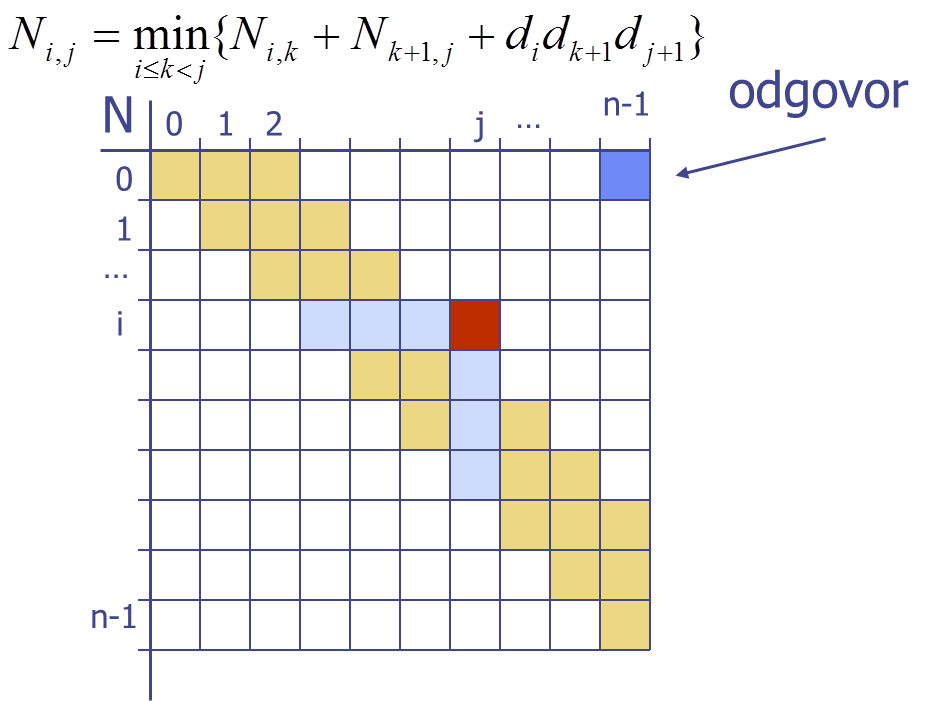
\includegraphics[width=6cm]{asp-13-pic09.png}
      \end{center}
    \end{column}
  \end{columns}
\end{frame}

\begin{frame}[fragile]
  \frametitle{Opšti postupak dinamičkog programiranja}
  \begin{itemize}
    \item primenljivo na probleme čije rešavanje traži puno vremena 
    (moguće eksponencijalni) ukoliko postoje:
    \begin{itemize}
      \item \myred{jednostavni potproblemi}: potproblemi se mogu 
      definisati pomoću promenljivih $j,k,l,m$ itd.
      \item \myred{optimalni potproblemi}: globalni optimum se može 
      definisati pomoću optimalnih potproblema
      \item \myred{preklapanje potproblema}: potproblemi nisu nezavisni
      i treba ih konstruisati bottom-up
    \end{itemize}
  \end{itemize}
\end{frame}

\begin{frame}[fragile]
  \frametitle{Podsekvence}
  \begin{itemize}
    \item \myred{podsekvenca} stringa $x_{0}x_{1}x_{2}\ldots x_{n-1}$ je
    string $x_{i_{1}}x_{i_{2}}\ldots x_{i_{k}}$ gde je $i_{j}<i_{j+1}$
    \item nije isto što i podstring!
    \item primer stringa: ABCDEFGHIJK
    \begin{itemize}
      \item jeste podsekvenca: ACEGIJK
      \item jeste podsekvenca: DFGHK
      \item nije podsekvenca: DAGH
    \end{itemize}
  \end{itemize}
\end{frame}

\begin{frame}[fragile]
  \frametitle{Problem najduže zajedničke podsekvence}
  \begin{itemize}
    \item \myred{longest common subsequence} (LCS)
    \item za stringove $X$ i $Y$, LCS je najduža podsekvenca od $X$ i $Y$
    \item primena: ispitivanje sličnosti DNK (alfabet je \{A,C,G,T\})
    \item primer: ABCDEFG i XZACKDFWGH imaju LCS: ACDFG
  \end{itemize}
\end{frame}

\begin{frame}[fragile]
  \frametitle{LCS grubom silom}
  \begin{itemize}
    \item primena grube sile na LCS:
    \begin{itemize}
      \item pronađi sve podsekvence od $X$
      \item izdvoj one koje su i podsekvence od $Y$
      \item izaberi najdužu
    \end{itemize}
    \item analiza:
    \begin{itemize}
      \item ako je $X$ dužine $n$, ima $2^n$ podsekvenci
      \item ovo je eksponencijalno vreme!
    \end{itemize}
  \end{itemize}
\end{frame}

\begin{frame}[fragile]
  \frametitle{LCS dinamičkim programiranjem}
  \begin{itemize}
    \item neka je $L[i,j]$ LCS za $X[0..i]$ i $Y[0..j]$
    \item neka postoji indeks -1, tako da je $L[-1,k]=0$ i $L[k,-1]=0$; 
    to znači da null deo X ili Y nema poklapanja sa drugim
    \item sada definišemo $L[i,j]$ u opštem slučaju:
    \begin{itemize}
      \item ako je $x_{i}=y_{j}$ onda $L[i,j] = L[i-1,j-1]+1$ \\ (imamo poklapanje)
      \item ako je $x_{i}\neq y_{j}$ onda $L[i,j] = \max\{L[i-1,j], L[i,j-1]\}$ \\ (nemamo poklapanje)
    \end{itemize}
  \end{itemize}
  \begin{center}
    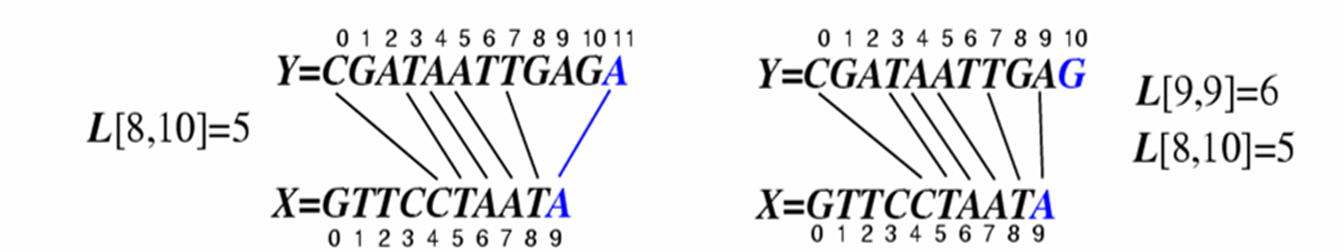
\includegraphics[width=11cm]{asp-13-pic10.png}
  \end{center}
\end{frame}

\begin{frame}[fragile,shrink]
  \frametitle{LCS algoritam}
  \myred{LCS}($X,Y$)
  \begin{algorithmic}
    \REQUIRE stringovi $X$ i $Y$ dužine $n$ odnosno $m$
    \ENSURE $L[i,j]$ za $0\leq i<n$ i $0\leq j<m$
    \FOR{$i \leftarrow 0$ \TO $n-1$}
      \STATE $N_{i,-1} \leftarrow 0$
    \ENDFOR
    \FOR{$j \leftarrow 0$ \TO $m-1$}
      \STATE $N_{-1,j} \leftarrow 0$
    \ENDFOR
    \FOR{$i \leftarrow 0$ \TO $n-1$}
      \FOR{$j \leftarrow 0$ \TO $m-1$}
        \IF{$x_{i} = y_{j}$}
          \STATE $L[i,j] \leftarrow L[i-1,j-1]+1$
        \ELSE
          \STATE $L[i,j] \leftarrow \max\{L[i-1,j], L[i,j-1]\}$
        \ENDIF
      \ENDFOR
    \ENDFOR
    \RETURN $L$
  \end{algorithmic}    
\end{frame}

\begin{frame}[fragile]
  \frametitle{LCS algoritam: vizuelizacija}
  \begin{center}
    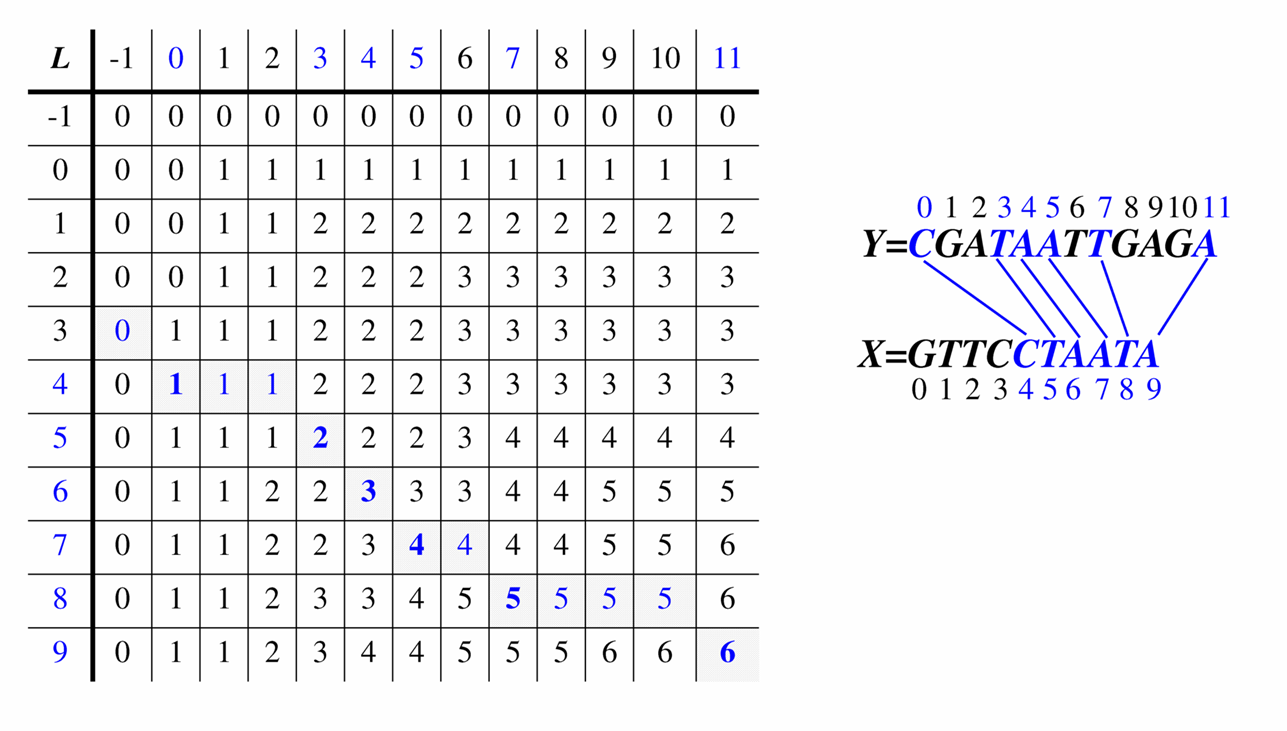
\includegraphics[width=11cm]{asp-13-pic11.png}
  \end{center}
\end{frame}

\begin{frame}[fragile]
  \frametitle{LCS algoritam: analiza}
  \begin{itemize}
    \item algoritam ima dve ugnježdene petlje
    \begin{itemize}
      \item spoljna ima $n$ ciklusa
      \item unutrašnja ima $m$ ciklusa
      \item telo unutrašnje petlje ima konstantno vreme
      \item $\Rightarrow$ ukupno vreme je $O(nm)$
    \end{itemize}
    \item odgovor je sačuvan u $L[n,m]$
  \end{itemize}
\end{frame}

\begin{frame}[fragile,shrink=10]
  \frametitle{Python implementacija $_1$}
\begin{minted}[linenos=false]{python}
def LCS(X, Y):
  """Return table such that L[j][k] is 
     length of LCS for X[0:j] and Y[0:k].
     """
  n, m = len(X), len(Y)                
  L = [[0] * (m+1) for k in range(n+1)] # (n+1) x (m+1) table
  for j in range(n):
    for k in range(m):
      if X[j] == Y[k]:              # align this match
        L[j+1][k+1] = L[j][k] + 1            
      else:                         # choose to ignore one char
        L[j+1][k+1] = max(L[j][k+1], L[j+1][k])
  return L
\end{minted}
\end{frame}

\begin{frame}[fragile,shrink=10]
  \frametitle{Python implementacija $_2$}
\begin{minted}[linenos=false]{python}
def LCS_solution(X, Y, L):
  """Return the longest common substring 
     of X and Y, given LCS table L.
     """
  solution = []
  j,k = len(X), len(Y)
  while L[j][k] > 0:  # common characters remain
    if X[j-1] == Y[k-1]:
      solution.append(X[j-1])
      j -= 1
      k -= 1
    elif L[j-1][k] >= L[j][k-1]:
      j -=1
    else:
      k -= 1
  return ''.join(reversed(solution)) # return left-to-right 
                                     # version
\end{minted}
\end{frame}

\section[Pohlepa]{Pohlepni metod}

\begin{frame}[fragile]
  \frametitle{Pohlepna metoda}
  \begin{itemize}
    \item \myred{pohlepna metoda} je pristup dizajnu algoritama zasnovan
    na:
    \begin{itemize}
      \item \textbf{konfiguracije}: različiti izbori, kolekcije ili 
      vrednosti koje treba pronaći
      \item \textbf{funkcija cilja}: vrednost (\textit{score}) dodeljena
      konfiguracijama koju želimo da minimizujemo ili maksimizujemo
    \end{itemize}
    \item najbolje funkcioniše za probleme koji imaju osobinu 
    \myred{pohlepnog izbora}:
    \begin{itemize}
      \item globalno optimalno rešenje se može pronaći serijom lokalnih 
      unapređenja polazeći od početne konfiguracije
    \end{itemize}
  \end{itemize}
\end{frame}

\begin{frame}[fragile]
  \frametitle{Kompresija teksta}
  \begin{itemize}
    \item dati string $X$ zapiši/kodiraj kao $Y$ tako da $Y$ zauzima 
    manje memorije 
    \begin{itemize}
      \item štedi memoriju i/ili propusni opseg mreže
    \end{itemize}
    \item odličan primer: \myred{Huffman-ovo kodiranje} 
    \begin{itemize}
      \item izračunaj frekvenciju pojavljivanja svakog znaka
      \item najčešće znakove kodiraj najkraćim kodovima
      \item nijedan kôd nije prefiks nekog drugog
      \item koristi optimalno stablo kodiranja za određivanje kodova
    \end{itemize}
  \end{itemize}
\end{frame}

\begin{frame}[fragile]
  \frametitle{Stablo kodiranja}
  \begin{itemize}
    \item \myred{kôd} je preslikavanje karaktera iz alfabeta na binarni 
    reprezent -- kodnu reč
    \item \myred{prefiksni kôd} je takav binarni kôd da nijedna kodna 
    reč nije prefiks druge kodne reči
    \item \myred{stablo kodiranja} predstavlja prefiksni kôd
    \begin{itemize}
      \item listovi čuvaju karaktere iz alfabeta
      \item kodna reč dobija se obilaskom putanje od korena do lista
      \item 0 za levo dete i 1 za desno dete
    \end{itemize}
  \end{itemize}
  \begin{center}
    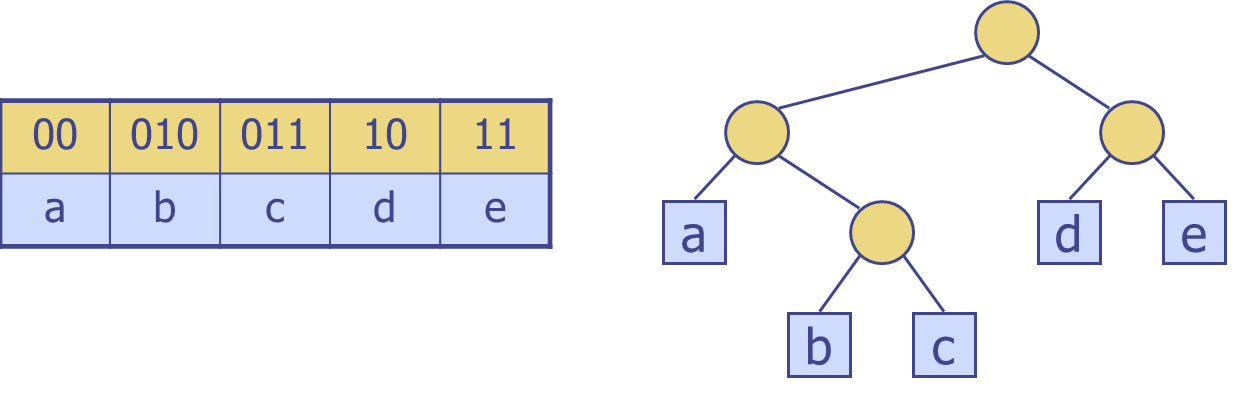
\includegraphics[width=10cm]{asp-13-pic12.png}
  \end{center}
\end{frame}

\begin{frame}[fragile]
  \frametitle{Optimizacija stabla kodiranja}
  \begin{itemize}
    \item za dati string $X$ tražimo prefiksni kod takav da rezultat 
    kompresije bude što kraći
    \begin{itemize}
      \item česti karakteri treba da imaju kratke kodne reči
      \item retki karakteri mogu da imaju duže kodne reči
    \end{itemize}
    \item primer:
    \begin{itemize}
      \item $X = abracadabra$
      \item $T_{1}$ kodira $X$ u 29 bita
      \item $T_{2}$ kodira $X$ u 24 bita
    \end{itemize}
  \end{itemize}
  \begin{center}
    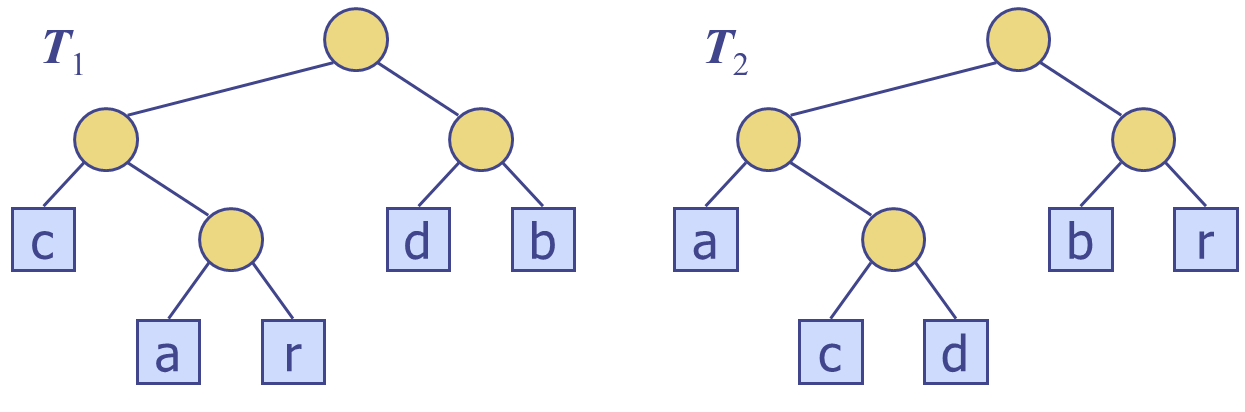
\includegraphics[width=10cm]{asp-13-pic13.png}
  \end{center}
\end{frame}

\begin{frame}[fragile]
  \frametitle{Huffman-ovo kodiranje}
  \begin{itemize}
    \item za dati string $X$ Huffman-ovo kodiranje konstruiše prefiksni 
    kod koji minimizuje dužinu kôda od $X$
    \item radi u $O(n + d\log d)$ vremenu
    \begin{itemize}
      \item $n$ je dužina $X$ 
      \item $d$ je veličina alfabeta
    \end{itemize}
    \item pomoćna struktura podataka: red sa prioritetom implementiran pomoću heapa
  \end{itemize}
\end{frame}

\begin{frame}[fragile,shrink]
  \frametitle{Huffman-ov algoritam}
  \myred{Huffman}($X$)
  \begin{algorithmic}
    \REQUIRE string $X$ dužine $n$ sa $d$ različitih znakova
    \ENSURE stablo kodiranja za $X$
    \STATE izračunaj frekvenciju $f(c)$ za svaki znak $c$ iz $X$
    \STATE $Q$ je novi red sa prioritetom
    \FORALL{$c \in X$}
      \STATE kreiraj koren stabla $T$ koji čuva $c$
      \STATE dodaj $T$ u $Q$ sa ključem $f(c)$
    \ENDFOR
    \WHILE{len($Q$)$>1$}
      \STATE $(f_{1},T_{1}) \leftarrow Q$.remove\_min()
      \STATE $(f_{2},T_{2}) \leftarrow Q$.remove\_min()
      \STATE kreiraj novo stablo $T$ sa levim podstablom $T_{1}$ i desnim $T_{2}$
      \STATE dodaj $T$ u $Q$ sa ključem $f_{1} + f_{2}$
    \ENDWHILE
    \STATE $(f,T) \leftarrow Q$.remove\_min()
    \RETURN $T$
  \end{algorithmic}    
\end{frame}

\begin{frame}[fragile]
  \frametitle{Huffman: primer 1}
  \begin{center}
    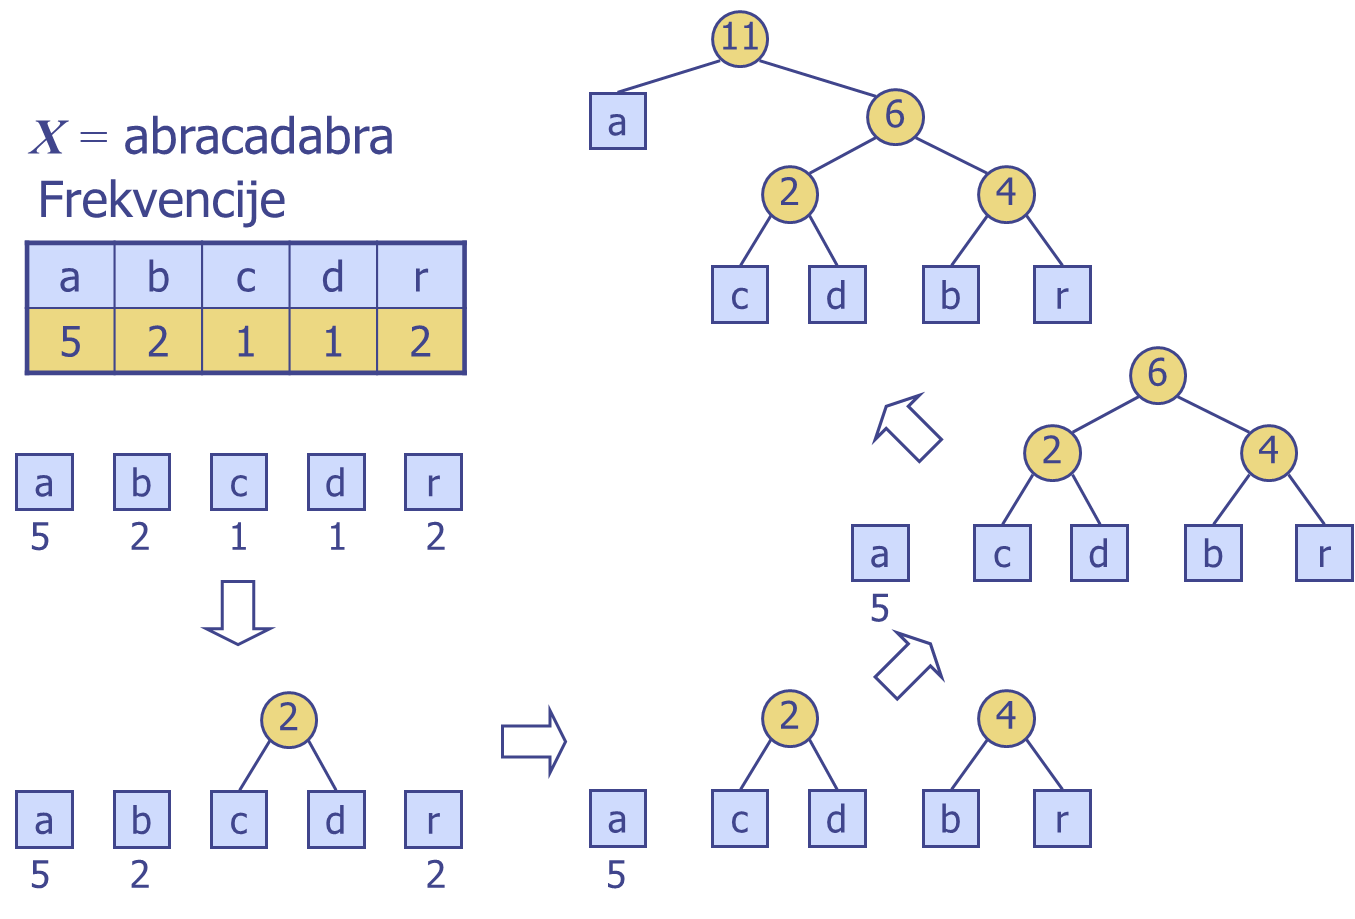
\includegraphics[width=10cm]{asp-13-pic14.png}
  \end{center}
\end{frame}

\begin{frame}[fragile]
  \frametitle{Huffman: primer 2}
  \begin{center}
    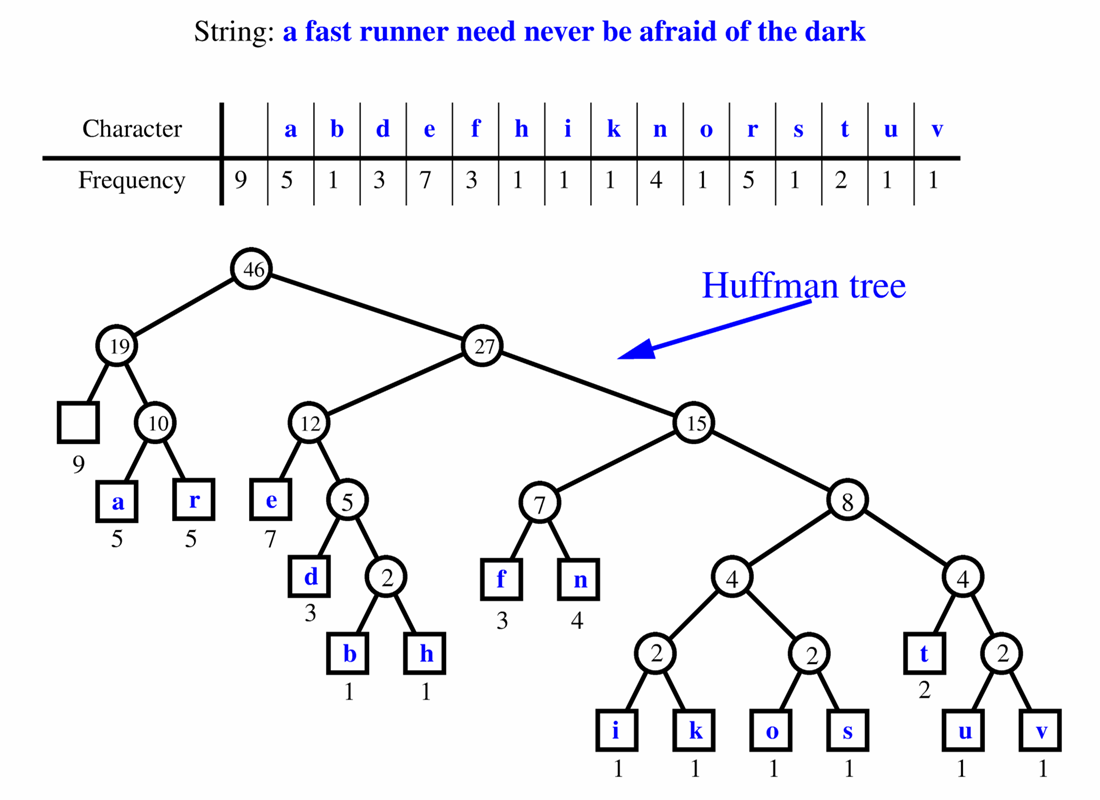
\includegraphics[width=10cm]{asp-13-pic15.png}
  \end{center}
\end{frame}

\begin{frame}[fragile]
  \frametitle{Problem ranca}
  \begin{itemize}
    \item dat je skup $S$ od $n$ elemenata, svaki element $i$ ima
    \begin{itemize}
      \item $b_{i}$ cenu (benefit)
      \item $w_{i}$ težinu
    \end{itemize}
    \item \textbf{cilj}: izaberi elemente sa maksimalnom ukupnom 
    vrednošću ali ukupnom težinom ne većom od $W$
  \end{itemize}
  \begin{center}
    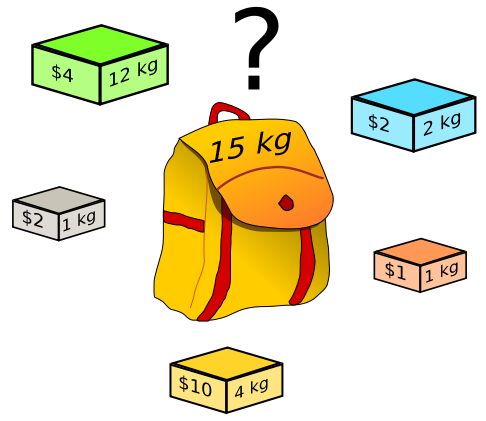
\includegraphics[width=5cm]{asp-13-pic28.png}
  \end{center}
\end{frame}

\begin{frame}[fragile]
  \frametitle{Problem ranca}
  \begin{itemize}
    \item ako je moguće uzeti razlomljene količine elemenata:
    \begin{itemize}
      \item $x_{i}$ je količina elementa $i$
      \item cilj: maksimizovati
      $$ \sum_{i\in S}b_{i}\frac{x_{i}}{w_{i}}$$
      \item uz ograničenje:
      $$ \sum_{i\in S} \leq W$$
    \end{itemize}
  \end{itemize}
\end{frame}

\begin{frame}[fragile]
  \frametitle{Problem ranca: primer}
  \begin{center}
    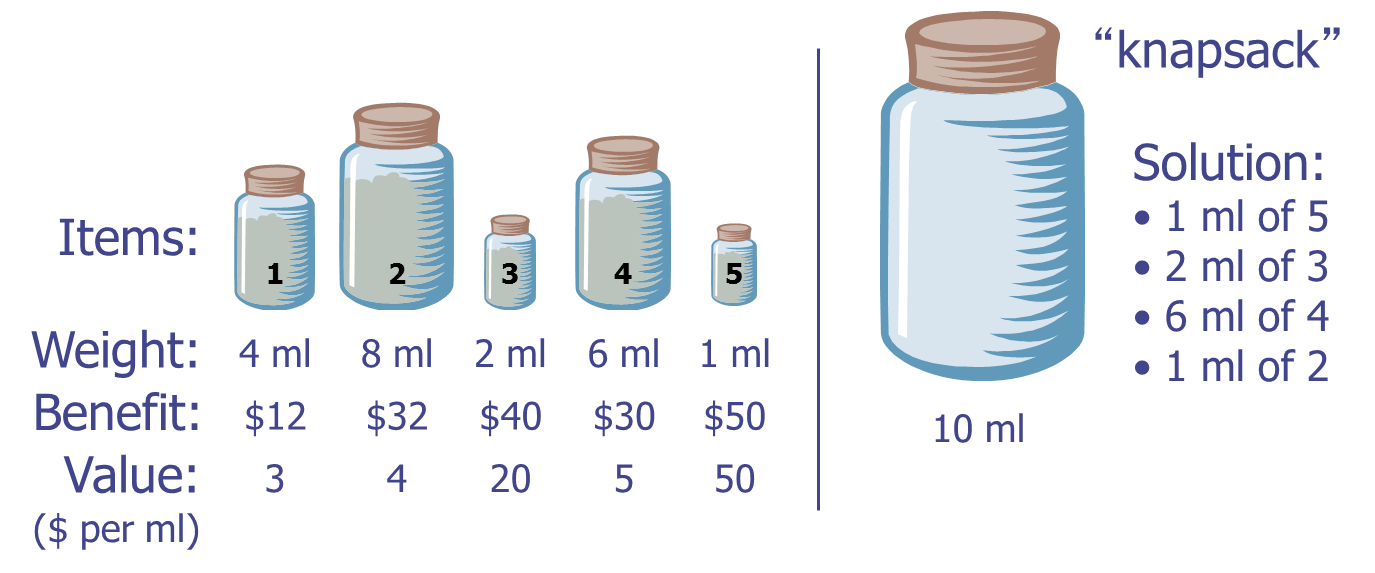
\includegraphics[width=10cm]{asp-13-pic16.png}
  \end{center}
\end{frame}

\begin{frame}[fragile]
  \frametitle{Problem ranca: algoritam}
  \begin{itemize}
    \item pohlepni izbor: izaberi element sa najvećom vrednošću (cena/težina)
    \begin{itemize}
      \item pošto je $\sum_{i\in S}b_{i}(x_{i}/w_{i}) = \sum_{i\in S}(b_{i}/w_{i})x_{i}$
      \item radi u $O(n\log n)$ vremenu
    \end{itemize}
    \item \textbf{korektnost}: pretpostavimo da postoji bolje rešenje
    \begin{itemize}
      \item postoji element $i$ sa većom vrednošću od izabranog elementa 
      $j$ ali je $x_{i}<w_{i}$ i $v_{i}<v_{j}$
      \item ako zamenimo $i$ sa $j$ dobićemo bolje rešenje
      \item koliko od $i$: $\min\{w_{i}-x_{i},x_{j}\}$
      \item dakle, nema boljeg rešenja od pohlepnog
    \end{itemize}
  \end{itemize}
\end{frame}

\begin{frame}[fragile,shrink]
  \frametitle{Problem ranca: algoritam}
  \myred{fractionalKnapsack}($S, W$)
  \begin{algorithmic}
    \REQUIRE skup $S$ elemenata $w$ sa cenom $b_{i}$ i težinom $w_{i}$, max težina $W$
    \ENSURE količina $x_{i}$ elementa $i$ da se maksimizuje cena uz max težinu $W$
    \FORALL{$i \in S$}
      \STATE $x_{i} \leftarrow 0$
      \STATE $v_{i} \leftarrow b_{i} / w_{i}$ \COMMENT{vrednost}
    \ENDFOR
    \STATE $w \leftarrow 0$ \COMMENT{ukupna težina}
    \WHILE{$w<W$}
      \STATE ukloni element $i$ sa najvećim $v_{i}$
      \STATE $x_{i} \leftarrow \min\{w_{i}, W-w\}$
      \STATE $w \leftarrow w + \min\{w_{i}, W-w\}$ 
    \ENDWHILE
  \end{algorithmic}    
\end{frame}

\begin{frame}[fragile]
  \frametitle{Raspoređivanje zadataka}
  \begin{itemize}
    \item za dati skup $T$ od $n$ zadataka svaki zadatak ima
    \begin{itemize}
      \item vreme početka $s_{i}$
      \item vreme završetka $f_{i}$ (gde je $s_{i}<f_{i}$)
    \end{itemize}
    \item \textbf{cilj}: obaviti sve zadatke sa minimalnim brojem mašina
  \end{itemize}
  \begin{center}
    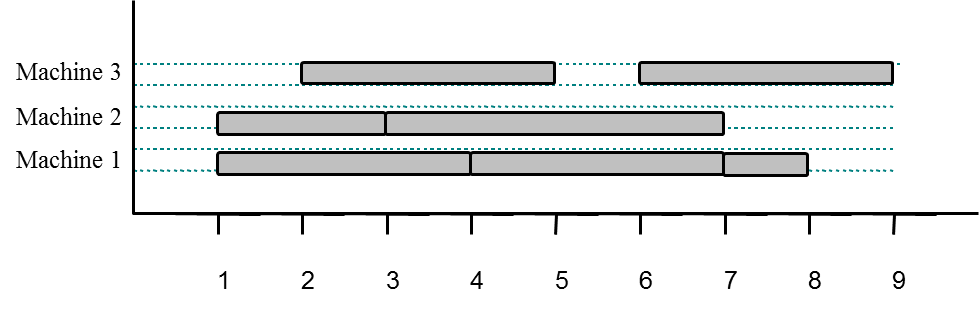
\includegraphics[width=10cm]{asp-13-pic17.png}
  \end{center}
\end{frame}

\begin{frame}[fragile]
  \frametitle{Raspoređivanje zadataka: algoritam}
  \begin{itemize}
    \item pohlepni izbor: razmatraćemo zadatke po vremenu početka i
    koristiti što manje mašina za ovaj redosled
    \begin{itemize}
      \item vreme izvršavanja $O(n\log n)$
    \end{itemize}
    \item \textbf{korektnost}: pretpostavimo da postoji bolji raspored
    \begin{itemize}
      \item možemo koristiti $k-1$ mašina
      \item alogritam koristi $k$
      \item neka je $i$ prvi zadatak planiran u postrojenju $k$
      \item mašina $i$ mora biti u konfliktu sa $k-1$ drugih zadataka
      \item ali to znači da postoji konzistentan raspored koji koristi
      $k-1$ mašina
    \end{itemize}
  \end{itemize}
\end{frame}

\begin{frame}[fragile,shrink]
  \frametitle{Raspoređivanje zadataka: algoritam}
  \myred{taskSchedule}($T$)
  \begin{algorithmic}
    \REQUIRE skup $T$ zadataka sa startnim vremenom $s_{i}$ i vremenom završetka $f_{i}$
    \ENSURE raspored sa minimalnim brojem mašina
    \STATE $m \leftarrow 0$ \COMMENT{broj mašina}
    \WHILE{$T$ nije prazan}
      \STATE ukloni zadatak $i$ sa najmanjim $s_{i}$
      \IF{postoji mašina $j$ za zadatak $i$}
        \STATE rasporedi zadatak $i$ na mašinu $j$
      \ELSE
        \STATE $m \leftarrow m+1$
        \STATE rasporedi zadatak $i$ na mašinu $m$
      \ENDIF
    \ENDWHILE
  \end{algorithmic}    
\end{frame}

\begin{frame}[fragile]
  \frametitle{Raspoređivanje zadataka: primer}
  \begin{itemize}
    \item za dati skup $T$ od $n$ zadataka, svaki zadatak ima
    \begin{itemize}
      \item vreme početka $s_{i}$
      \item vreme završetka $f_{i}$ (gde je $s_{i}<f_{i}$)
    \end{itemize}
    \item \textbf{primer}: $[1,4],[1,3],[2,5],[3,7],[4,7],[6,9],[7,8]$
    \item izvršiti zadatke na minimalnom broju mašina
  \end{itemize}
  \begin{center}
    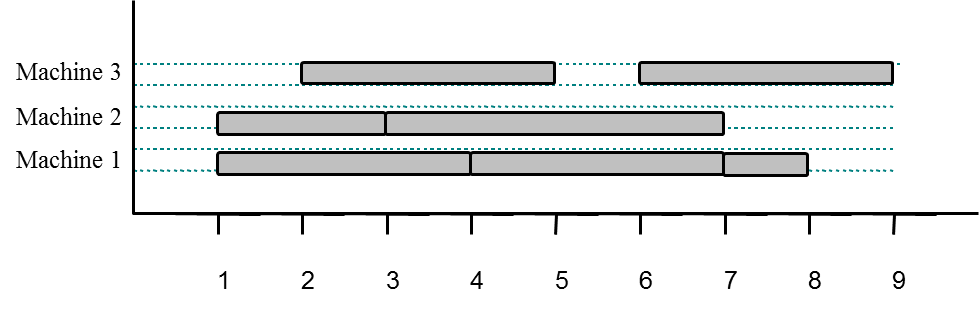
\includegraphics[width=10cm]{asp-13-pic17.png}
  \end{center}
\end{frame}

\section[Trie]{Trie}

\begin{frame}[fragile]
  \frametitle{Predprocesiranje stringova}
  \begin{itemize}
    \item predprocesiranje šablona ubrzava pattern matching
    \begin{itemize}
      \item vreme za KMP je proporcionalno dužini teksta nakon predprocesiranja
    \end{itemize}
    \item ako je tekst dugačak, ne menja se i često se pretražuje mogli bismo
    da predprocesiramo tekst umesto šablona
    \item \myred{trie} (čita se kao ,,try``) je struktura podataka za čuvanje
    stringova, npr. svih reči u tekstu
    \begin{itemize}
      \item vreme pretrage je proporcionalno dužini šablona
    \end{itemize}
  \end{itemize}
\end{frame}

\begin{frame}[fragile]
  \frametitle{Standardni trie}
  \begin{itemize}
    \item \myred{standardni trie} za skup stringova $S$ je stablo:
    \begin{itemize}
      \item svaki čvor osim korena čuva jedan karakter
      \item deca čvora su u alfabetskom redosledu
      \item putanja od korena do lista daje čuvani string
    \end{itemize}
    \item primer: S=\{bear, bell, bid, buy, sell, stock, stop\}
  \end{itemize}
  \begin{center}
    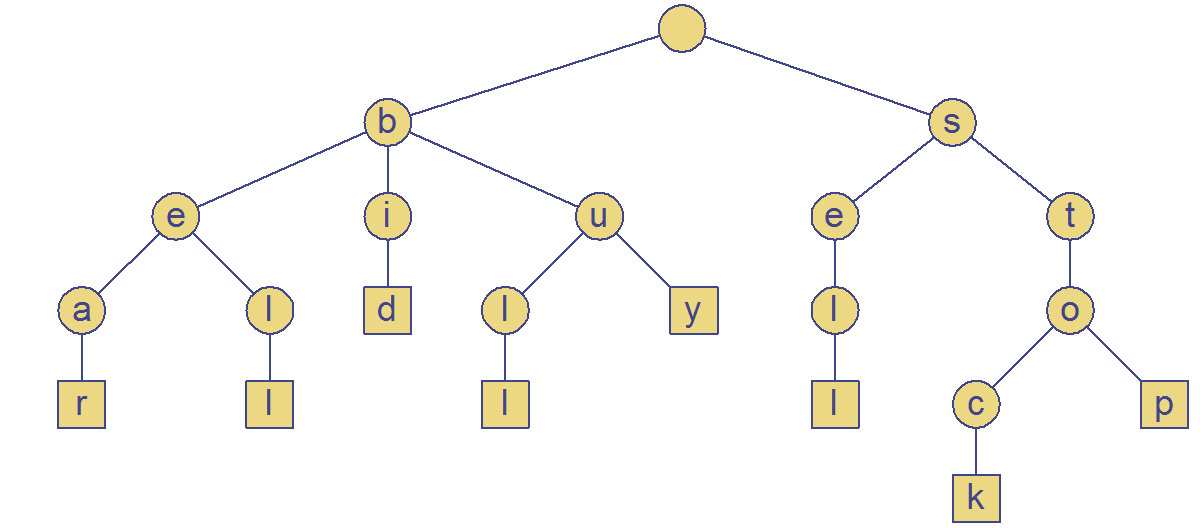
\includegraphics[width=10cm]{asp-13-pic18.png}
  \end{center}
\end{frame}

\begin{frame}[fragile]
  \frametitle{Standardni trie: analiza}
  \begin{itemize}
    \item standardni trie troši $O(n)$ prostora
    \item dodavanje, uklanjanje i pretraga su $O(dm)$
    \begin{itemize}
      \item $n$ ukupna dužina stringova u $S$
      \item $m$ dužina stringa u operaciji
      \item $d$ veličina alfabeta
    \end{itemize}
  \end{itemize}
  \begin{center}
    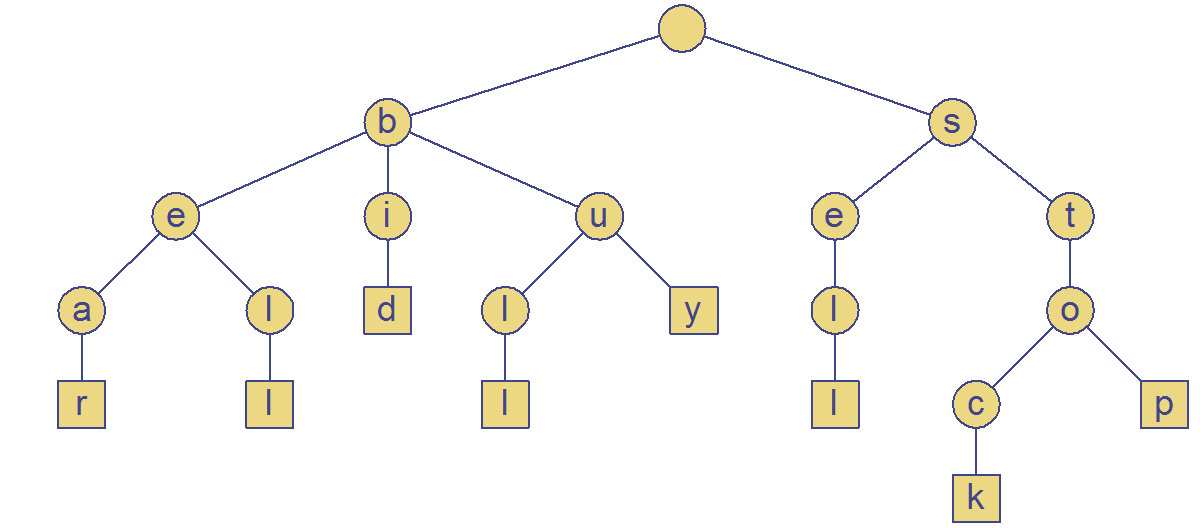
\includegraphics[width=10cm]{asp-13-pic18.png}
  \end{center}
\end{frame}

\begin{frame}[fragile]
  \frametitle{Traženje reči u trie}
  \begin{columns}
    \begin{column}[t]{4cm}
      {\footnotesize
      \begin{itemize}
        \item dodaj reči iz teksta u trie
        \item svaki list je jedna reč
        \item list čuva indekse gde počinje reč
      \end{itemize}}
    \end{column}
    \begin{column}[t]{8cm}
      \begin{center}
        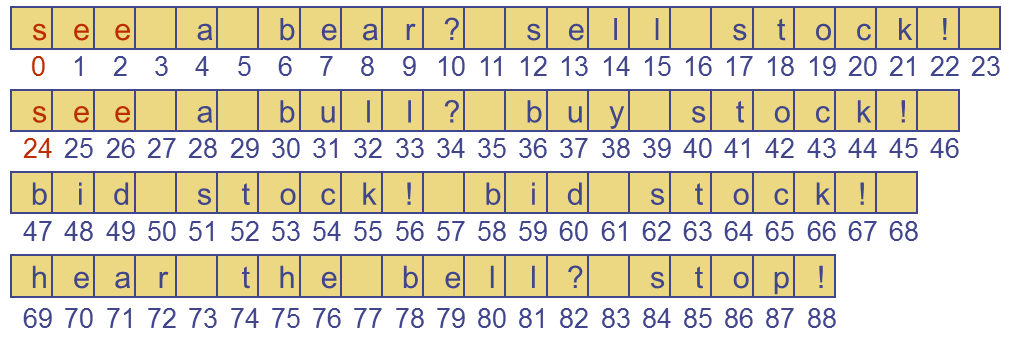
\includegraphics[width=7.5cm]{asp-13-pic19.png}
      \end{center}
    \end{column}
  \end{columns}
  \begin{center}
    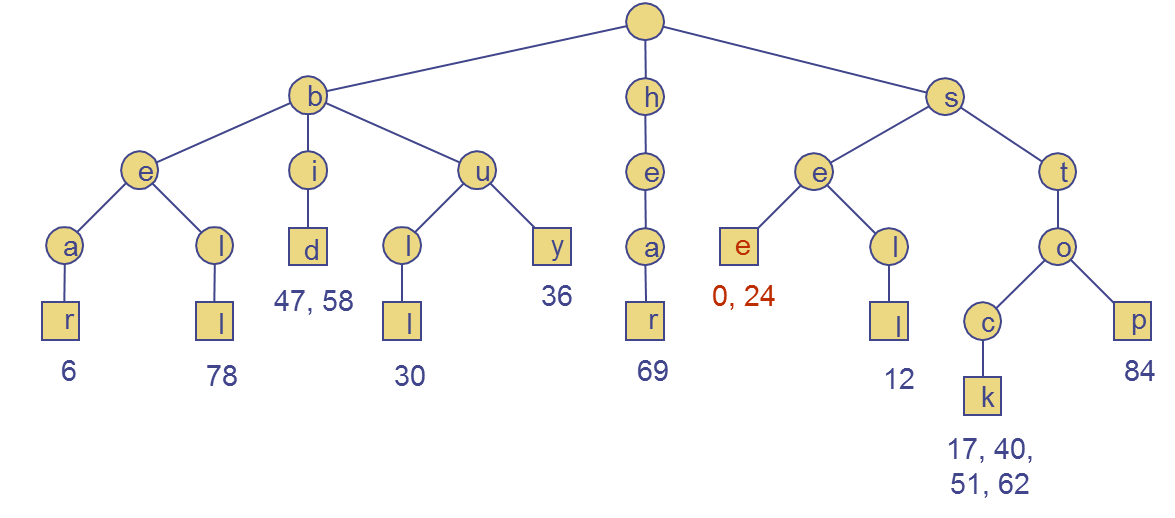
\includegraphics[width=10cm]{asp-13-pic20.png}
  \end{center}
\end{frame}

\begin{frame}[fragile]
  \frametitle{Kompresovani trie}
  \begin{center}
    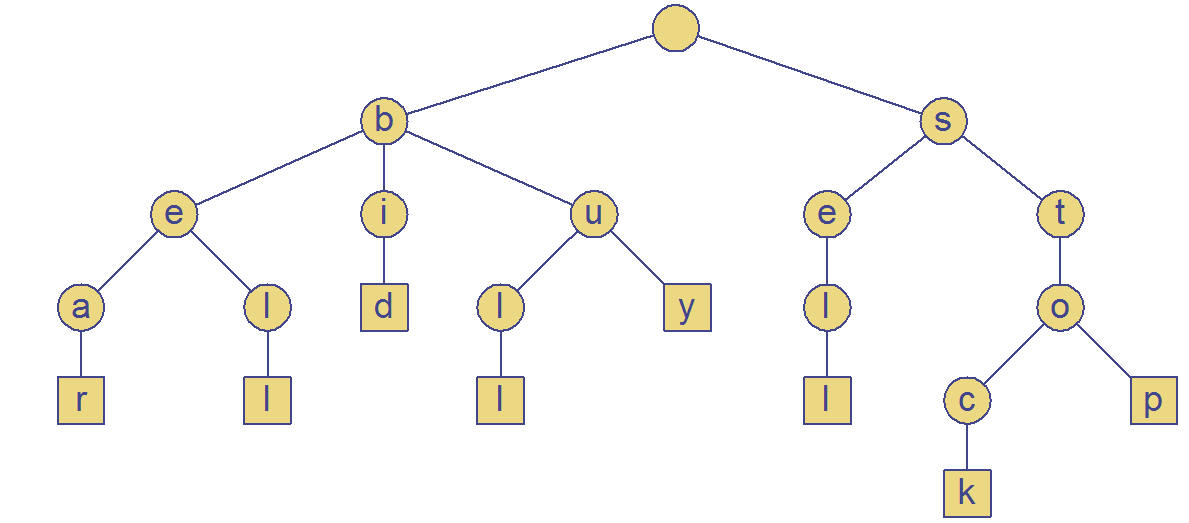
\includegraphics[width=9cm]{asp-13-pic21.png}
  \end{center}
  \begin{columns}
    \begin{column}[t]{5cm}
      {\footnotesize
      \begin{itemize}
        \item \myred{kompresovani trie} ima unutrašnje čvorove sa bar 2 deteta
        \item dobija se od standardnog kompresovanjem lanaca ,,redundantnih`` čvorova
      \end{itemize}}
    \end{column}
    \begin{column}[t]{7cm}
      \begin{center}
        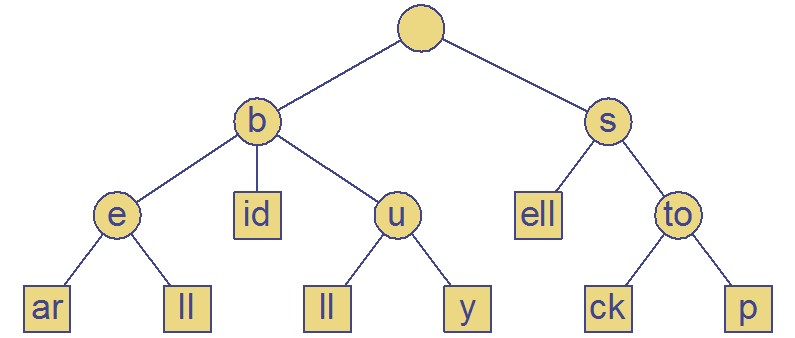
\includegraphics[width=6cm]{asp-13-pic22.png}
      \end{center}
    \end{column}
  \end{columns}
\end{frame}

\begin{frame}[fragile]
  \frametitle{Kompaktna reprezentacija}
  \begin{itemize}
    \item kompaktna reprezentacija kompresovanog trie-a za niz stringova
    \begin{itemize}
      \item čvorovi čuvaju opsege indeksa umesto podstringove
      \item troši $O(s)$ prostora gde je $s$ broj stringova u nizu
      \item služi kao pomoćna indeksna struktura
    \end{itemize}
  \end{itemize}
  \begin{center}
    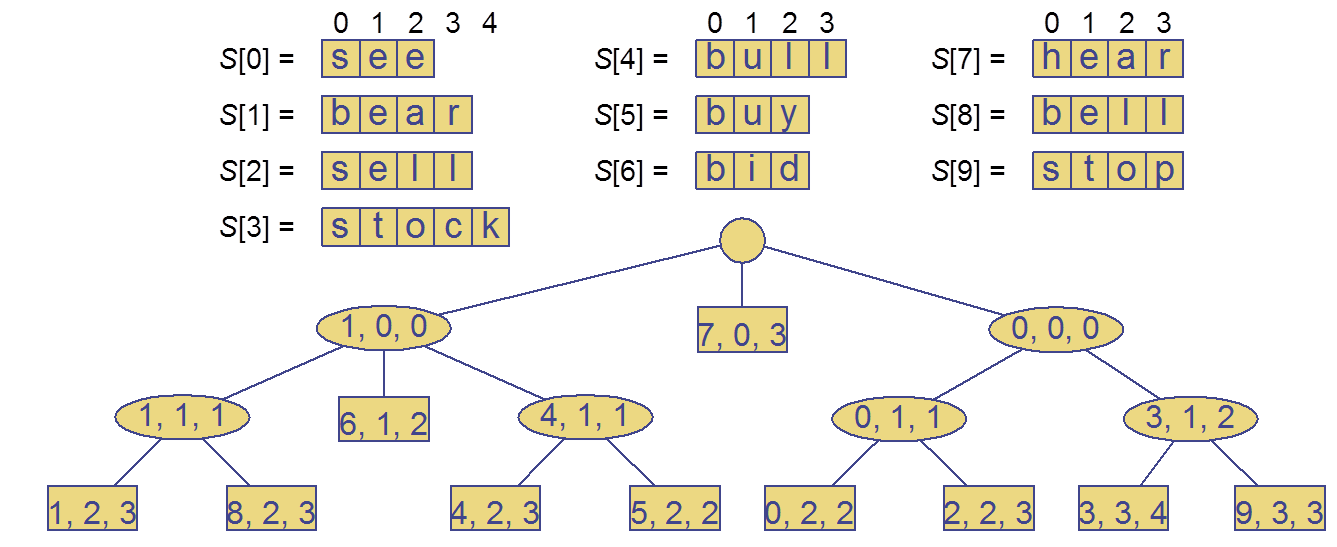
\includegraphics[width=11cm]{asp-13-pic23.png}
  \end{center}
\end{frame}

\begin{frame}[fragile]
  \frametitle{Sufiksni trie}
  \begin{itemize}
    \item \myred{sufiksni trie} stringa $X$ je kompresovani trie svih sufiksa od $X$
  \end{itemize}
  \begin{center}
    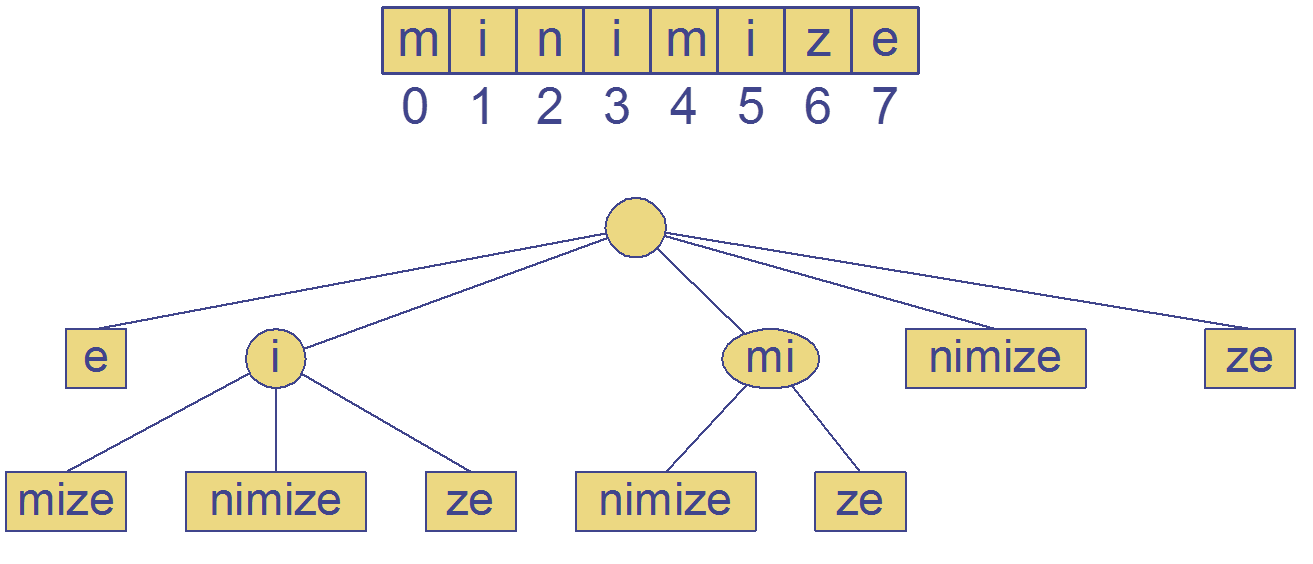
\includegraphics[width=11cm]{asp-13-pic24.png}
  \end{center}
\end{frame}

\begin{frame}[fragile]
  \frametitle{Sufiksni trie: analiza}
  \begin{itemize}
    \item string $X$ dužine $n$, alfabet veličine $d$
    \begin{itemize}
      \item troši $O(n)$ prostora
      \item pretraga za $O(dm)$ vreme; $m$ dužina traženog šablona
      \item konstruiše se za $O(n)$ vreme
    \end{itemize}
  \end{itemize}
  \begin{center}
    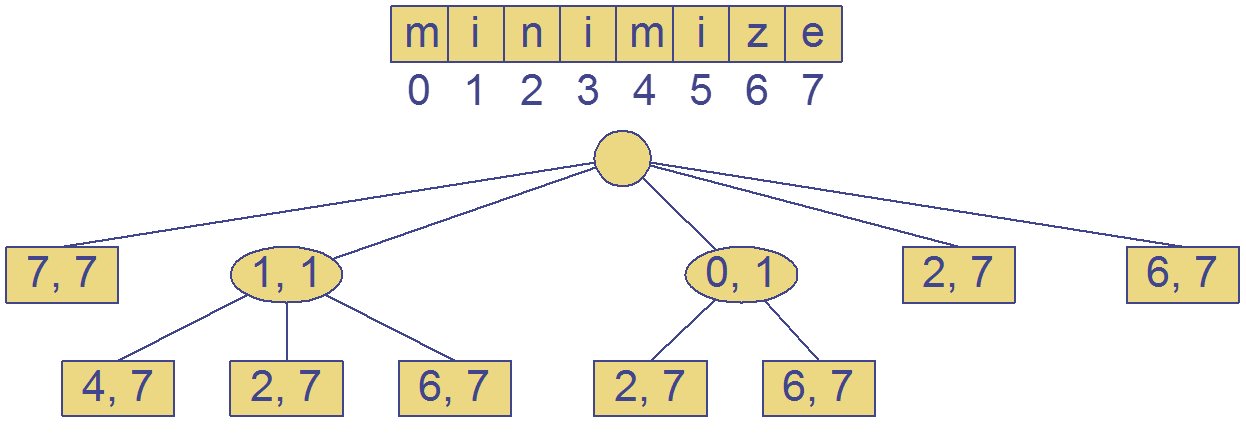
\includegraphics[width=10cm]{asp-13-pic25.png}
  \end{center}
\end{frame}

\begin{frame}[fragile]
  \frametitle{Kodni trie}
  \begin{itemize}
    \item \myred{kodni trie} predstavlja prefiksni kod
    \begin{itemize}
      \item svaki list čuva karakter
      \item kodna reč predstavlja putanju od korena do lista
      \item 0 za levo dete, 1 za desno dete
    \end{itemize}
  \end{itemize}
  \begin{center}
    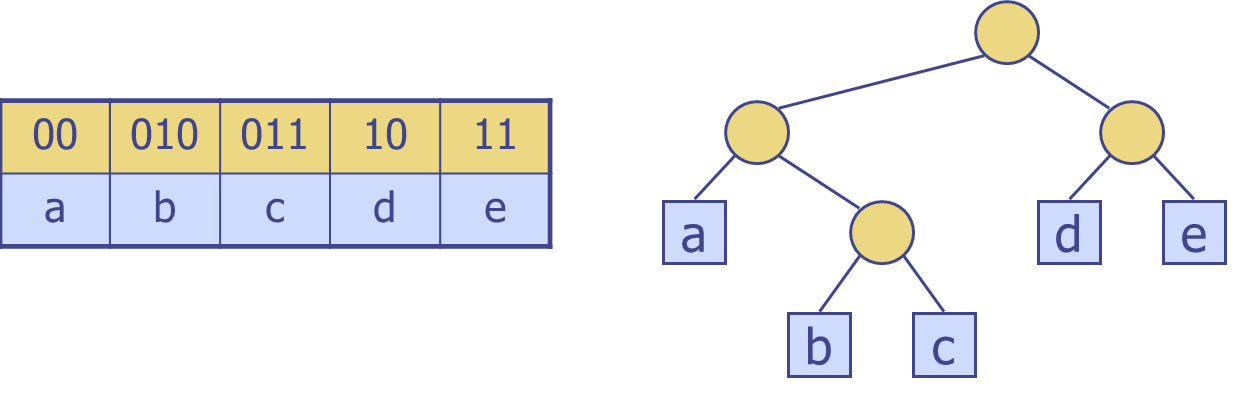
\includegraphics[width=10cm]{asp-13-pic26.png}
  \end{center}
\end{frame}

\begin{frame}[fragile]
  \frametitle{Kodni trie}
  \begin{itemize}
    \item za dati string $X$ tražimo prefiksni kod takav da rezultat 
    kompresije bude što kraći
    \begin{itemize}
      \item česti karakteri treba da imaju kratke kodne reči
      \item retki karakteri mogu da imaju duže kodne reči
    \end{itemize}
    \item primer:
    \begin{itemize}
      \item $X = abracadabra$
      \item $T_{1}$ kodira $X$ u 29 bita
      \item $T_{2}$ kodira $X$ u 24 bita
    \end{itemize}
  \end{itemize}
  \begin{center}
    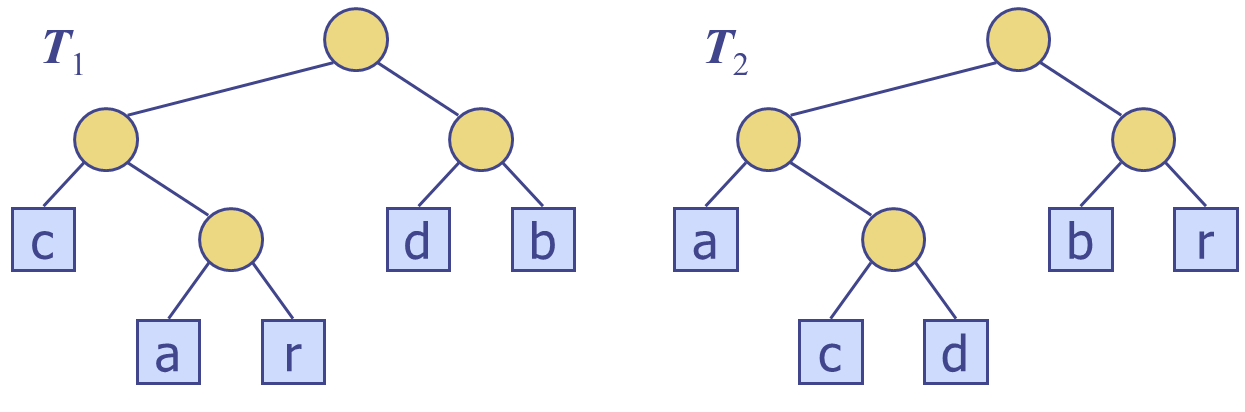
\includegraphics[width=10cm]{asp-13-pic27.png}
  \end{center}
\end{frame}

\end{document}
